
\documentclass[a4paper,fleqn,usenatbib]{mnras}

\usepackage{newtxtext,newtxmath}
% Depending on your LaTeX fonts installation, you might get better results with one of these:
%\usepackage{mathptmx}
%\usepackage{txfonts}

\usepackage[T1]{fontenc}
\usepackage{ae,aecompl}


\usepackage{graphicx}	% Including figure files
\usepackage{amsmath}	% Advanced maths commands
\usepackage{amssymb}	% Extra maths symbols

\makeatletter
\newcommand{\rmnum}[1]{\romannumeral #1}
\newcommand{\Rmnum}[1]{\expandafter\@slowromancap\romannumeral #1@}
\makeatother

\usepackage{color}
\newcommand{\todo}[1]{\textcolor{red}{#1}}


%%%%%%%%%%%%%%%%%%%%%%%%%%%%%%%%%%%%%%%%%%%%%%%%%%

%%%%% AUTHORS - PLACE YOUR OWN COMMANDS HERE %%%%%

% Please keep new commands to a minimum, and use \newcommand not \def to avoid
% overwriting existing commands. Example:
%\newcommand{\pcm}{\,cm$^{-2}$}	% per cm-squared

%%%%%%%%%%%%%%%%%%%%%%%%%%%%%%%%%%%%%%%%%%%%%%%%%%


% Title of the paper, and the short title which is used in the headers.
% Keep the title short and informative.
\title[Short title, max. 45 characters]{Man's not hot, Man can never be hot}

% The list of authors, and the short list which is used in the headers.
% If you need two or more lines of authors, add an extra line using \newauthor
\author[B. J. Norfolk et al.]{Brodie J. Norfolk,$^{1}$\thanks{E-mail: bjee7@student.monash.edu (MU)}
Andrew R. Casey,$^{1,2}$
Ernie? Kemp? Karakas? Lattanzio? \newauthor
Schlaufman? others?
\\
% List of institutions
$^{1}$School of Physics \& Astronomy, Monash University, Clayton 3800, Victoria, Australia\\
$^{2}$Faculty of Information Technology, Monash University, Clayton 3800, Victoria, Australia\\
}

\date{Accepted XXX. Received YYY; in original form ZZZ}

\pubyear{2018}

\begin{document}
\label{firstpage}
\pagerange{\pageref{firstpage}--\pageref{lastpage}}
\maketitle

\begin{abstract}
This is a simple template for authors to write new MNRAS papers.
The abstract should briefly describe the aims, methods, and main results of the paper.
It should be a single paragraph not more than 250 words (200 words for Letters).
No references should appear in the abstract.
\end{abstract}

\begin{keywords}
keyword1 -- keyword2 -- keyword3
\end{keywords}


\section{Introduction}

% What's a barium star (as observed)?% What causes a barium star? (extrinsic/intrinsic?)


Barium stars are chemically unusual red giants with an overabundance of carbon and heavy elements ($Z > 30$) relative to the Sun \citep{Bidelman1951}. \todo{Explain why this chemical signature is unusual: because this signature can really only be produced by TP-AGB stars, but we see barium stars that have not evolved to the AGB stars. Introduce extrinsic/intrinsic. Barium stars are considered to have been polluted by a binary TP-AGB star, or they are TP-AGB stars themselves.}


% AGB stars and the s-process.

About half of all heavy elements are produced by the slow neutron-capture process ($s$-process) inside asymptotic giant branch (AGB) stars \citep[e.g.][]{busso1999,travaglio2001,
herwig2005,romano2010,kobayashi2011,prantzos2012,bisterzo2014,
karakas12016}. 
\todo{This is very good, but the sentence needs splitting up: Late in the AGB phase, during the thermally pulsing-AGB (TP-AGB) phase, thermal instabilities occur in the He shell every $10^5$ years or so, depending on the H-exhausted core mass, and will drive a convective zone that sweeps the entire region lying between the core mass and He-shell; mixing the products of nucleosynthesis within these regions.} The energy from each thermal pulse forces the star to expand, pushing the H-shell out to cooler regions and allowing the convective envelope to move inwards to regions previously mixed by the thermally-driven convective zone. This expansion and resulting inward movement is described as the third dredge up (TDU), and is theorised to occur after every thermal pulse. 
The repeated downwash extensions of TDU cause enhancement of surface $^{12}$C abundance and of other heavy elements produced by the s-process \citep[e.g.,][]{busso2001}. The star contracts after \todo{PDU} and reignites the H-shell, producing the majority of the surface luminosity for the next interpulse period. The interpulse, thermal pulse, and dredge up cycle may occur numerous times and is dependent on the initial mass, composition, and mass-loss rate of the star.


Barium giants form within a metallicity dependent initial mass range (approximately 0.8 - 8$M_{\odot}$), with the minimum mass for core helium and carbon burning decreasing as metalicity decreases. The age of these stars vary considerably, with observable stars in metal-poor globular clusters hosting populations of $\approx$12Gyr. In contrast, metal rich, young observable stars reaching the upper limit may only reach $\approx$100Myr, this includes stars that are at the core carbon burning limit or very close to it \citep[e.g.][]{whitelock2013}.

% Comparisons to expectations of theoretical birth rate
% Binary fraction at different metallicities
% Mass differentials of binary stars
% Yields of AGB stars at different masses and metallicities.


According to the mass-transfer hypothesis, extrinsic Barium stars are a consequence of stellar wind accretion \citep{boffin1988,jorissen1992} or Roche-lobe overflow \citep{webbink1986}, and are within a binary system containing a previous AGB companion star (intrinsic Barium star) in its final phase as a white dwarf \citep{bohm1980,bohm1984}. In fact, \citet{mcclure1983} determines 85\% of all Barium stars are in binary systems and those that appear singular are actually pole-on, or highly eccentric binaries with significant radial velocity variations only occuring in a small phase range as detailed by \citet{pourbaix2004}.

Barium stars currently have only been discovered in the disk and halo of the Galaxy according to \citet{gomez1997} and \citet{mennessier1997}. Both studies show the stellar populations of Barium stars can be seperated into two groups when divided according to luminosity, kinematic and spatial parameters. Barium stars populating the halo have already been investigated \citep[e.g.][]{junqueira2001,drake2008,pereira2009,allen2006} and their relationship with metal-poor, yellow, symbiotic halo stars has been established by \citet{jorissen2005} and \citet{pereira2009}. Additionally, \citet{pereira2011} concludes metal-rich barium stars share similar kinematics to other metal-rich and super metal-rich stars already analysed, demonstrating they do not belong to the bulge population. Furthermore, it is neccessary to establish known abundances of s-process elements in a greater sample of Barium stars to conclude the percentage population of said stars in the Galaxy, and compare with their theoratical birthrate \citep{han1995}



\todo{The red giants studied here display especially strong s-process enhancement for \ion{Ba}{II} and \ion{Sr}{II} at lines 4554\AA\ and 4077\AA, respectively. (thinking I should extend this sentence with a little on the Carbon, maybe I should search for carbon in my figures ?). }

In this paper we analysis the \textit{Cannon} fitted LAMOST spectra \citep{ho2017} to obtain a sample set of s-process enriched Barium stars and investigate atmospheric parameters including, the distributions of temperature, surface gravity and metalicity. Additionally, the abundances of elements not produced in the s-process such as sodium and technetium (Na and Tc) are examined to determine  if the sample Barium stars share similar abundance to field giants with equal metallicities. Moreover, the stellar sample is cross matched with GAIA, producing (not sure exactly what gaia gave us) neccessary to determine the kinematics of our Barium samples. 

In our research we analysed 273 Barium canidates amoung the 454,180 stellar sample produced by \citet{ho2017} and with GAIA determined the galactic motions for 21 out the 273 canidates.

\section{Observations and Target Selection}
The spectral data of our stars were obtained from the \textit{Cannon} fits predictive model implemented by \citet{ho2017} on the LAMOST (Large Sky Area Multi-Object Fibre Spectroscopic Telescope) DR2 release \citep{luo2015}. The LAMOST spectral resolving power of R = 1800, a wavelength coverage from 3700$\AA$ to 9000$\AA$, and a nominal S/N ratio of 100. \citet{ho2017} cross-matches 9,952 stars between the low resolution spectra of LAMOST and the high resolution spectra from the APOGEE survey, and through a data driven spectral model. produces a 454,180 stellar data set. For this stellar data set the \textit{Cannon} predictive model infers $T_{eff}$, $log g$, $[Fe/H]$, and [$\alpha/M$] values.

The Barium stars analysed in this research were obtained by filtering for significant flux residuals, taken as, a disparity between the normalised LAMOST flux and the data driven model derived by \citet{ho2017}. A negative residual as shown in (I know I shoould expand here on the psoter child)figure \ref{fig:figure1} illustrates an enhancement in Ba\Rmnum{2} and Sr\Rmnum{2} at lines 4554\AA \hspace{0.2mm} and 4077\AA, respectively. (thinking a sentence on why these lines are the strongest ?). The filter process had five requirements that each spectra for both enhancement lines had to meet to be considered a Barium star canidate, these included:

\renewcommand\labelenumi{(\roman{enumi})}
\renewcommand\theenumi\labelenumi

\begin{enumerate} 
\item Profile amplitude for both enhancement lines must exceed A$\leq$-0.05.
\item Both amplittudes must be measured within 3$\sigma$ $(|A|/\sigma _A \geq 3)$.
\item The wavelength at each absorption line must be within $2$\AA \hspace{0.2mm}$(\lambda \leq 2)$.
\item The chi must be less then 3 (not sure on math wrting for this).
\item And, the spectra must have a signal-to-noise ratio of S/N $\geq 30$.
\end{enumerate}
In addition, a visual observation of the accuracy between each normalised LAMOST flux and its accompanying data driven model was undertaken to exclude any results containing, false positives, candidates exhibiting data reduction issues, apparent absorption finer then the spectral resolution, and overly noisy normalised LAMOST spectra. This combined method generated the 273 Barium star candidates as listed in Table \ref{table:table1}. 


\section{Analysis and Results}

\subsection{Line Selection}
\subsection{Technetium Lines}
\subsection{Abundance Analysis}
\subsection{Abundance Uncertainties}

\section{Discussion}

\section{Conclusions}

The last numbered section should briefly summarise what has been done, and describe
the final conclusions which the authors draw from their work.

\section*{Acknowledgements}

The Acknowledgements section is not numbered. Here you can thank helpful
colleagues, acknowledge funding agencies, telescopes and facilities used etc.
Try to keep it short.

%\section{Examples}
%
%Normally the next section describes the techniques the authors used.
%It is frequently split into subsections, such as Section~\ref{sec:maths} below.
%
%\subsection{Maths}
%\label{sec:maths} 
%
%Simple mathematics can be inserted into the flow of the text e.g. $2\times3=6$
%or $v=220$\,km\,s$^{-1}$, but more complicated expressions should be entered
%as a numbered equation:
%
%\begin{equation}
%    x=\frac{-b\pm\sqrt{b^2-4ac}}{2a}.
%	\label{eq:quadratic}
%\end{equation}
%
%Refer back to them as e.g. equation~(\ref{eq:quadratic}).
%
%\subsection{Figures and tables}
%
%Figures and tables should be placed at logical positions in the text. Don't
%worry about the exact layout, which will be handled by the publishers.
%
%Figures are referred to as e.g. Fig.~\ref{fig:example_figure}, and tables as
%e.g. Table~\ref{tab:example_table}.
%
%\begin{figure}
%	% To include a figure from a file named example.*
%	% Allowable file formats are eps or ps if compiling using latex
%	% or pdf, png, jpg if compiling using pdflatex
%	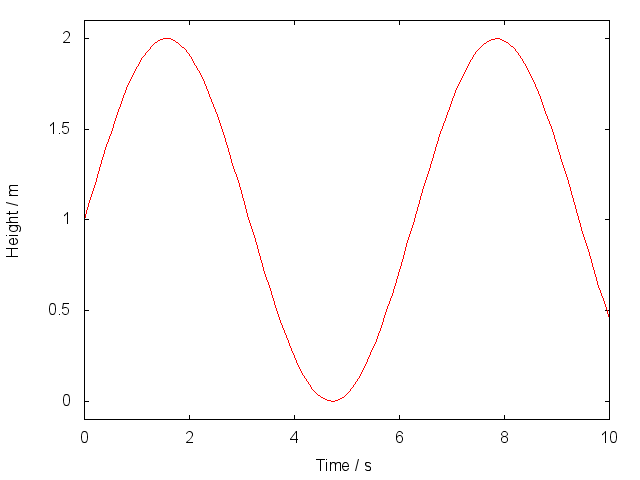
\includegraphics[width=\columnwidth]{example}
%    \caption{This is an example figure. Captions appear below each figure.
%	Give enough detail for the reader to understand what they're looking at,
%	but leave detailed discussion to the main body of the text.}
%    \label{fig:example_figure}
%\end{figure}
%
%
%\begin{table}
%	\centering
%	\caption{This is an example table. Captions appear above each table.
%	Remember to define the quantities, symbols and units used.}
%	\label{tab:example_table}
%	\begin{tabular}{lccr} % four columns, alignment for each
%		\hline
%		A & B & C & D\\
%		\hline
%		1 & 2 & 3 & 4\\
%		2 & 4 & 6 & 8\\
%		3 & 5 & 7 & 9\\
%		\hline
%	\end{tabular}
%\end{table}


% The best way to enter references is to use BibTeX:
 
\bibliographystyle{mnras}
\bibliography{example} % if your bibtex file is called example.bib

\begin{thebibliography}{99}
\bibitem[\protect\citeauthoryear{Author}{2012}]{Author2012}
Author A.~N., 2013, Journal of Improbable Astronomy, 1, 1
\bibitem[\protect\citeauthoryear{Others}{2013}]{Others2013}
Others S., 2012, Journal of Interesting Stuff, 17, 198


\bibitem[\protect\citeauthoryear{Bidelman \& Keenan}{1951}]{Bidelman1951}
Bidelman, W.~P. \& Keenan, P.~C. , 1951, ApJ, 114, 473
\bibitem[\protect\citeauthoryear{Busso et al.}{1999}]{busso1999}
Busso, M., Gallino, R., \& Wasserburg, P.~C. 1999, 
ARA$\&$A, 37, 239
\bibitem[\protect\citeauthoryear{Travaglio et al.}{2001}]{travaglio2001}
Travaglio, C., et al. 2001, 
ApJ, 549, 346
\bibitem[\protect\citeauthoryear{Herwig}{2005}]{herwig2005}
Herwig, F. 2005, 
ARA$\&$A, 43, 435
\bibitem[\protect\citeauthoryear{Romano et al.}{2010}]{romano2010}
Romano, D., et al. 2010, 
A$\&$A, 522, A32
\bibitem[\protect\citeauthoryear{Kobayashi et al.}{2011}]{kobayashi2011}
Kobayashi, C., Karakas, A., \& Umeda, H. 2011, 
MNRAS, 414, 3231
\bibitem[\protect\citeauthoryear{Prantzos}{2012}]{prantzos2012}
Prantzos, N. 2012, 
A$\&$A, 542, A67
\bibitem[\protect\citeauthoryear{Bisterzo et al.}{2014}]{bisterzo2014}
Bisterzo, S., et al. 2014, 
ApJ, 787, 10
\bibitem[\protect\citeauthoryear{Karakas}{2016}]{karakas12016}
Karakas, A. 2016, 
SAIt, 87, 229
\bibitem[\protect\citeauthoryear{Busso et al.}{2001}]{busso2001}
Busso, M., Gallino, R., Lambert, D.~L., Travaglio, C.\& Smith, V.~V. 2001, 
ApJ, 557, 802
\bibitem[\protect\citeauthoryear{McClure}{1983}]{mcclure1983}
McClure, R.~D. 1983, 
ApJ, 268, 264
\bibitem[\protect\citeauthoryear{Pourbaix et al.}{2004}]{pourbaix2004}
Pourbaix, D., Tokovinin, A.~A., Batten, A.~H., Fekel, F.~C., Hartkopf, W.~I. et al. 2001, 
A$\&$A, 424, 727
\bibitem[\protect\citeauthoryear{B\"ohm-Vitense}{1980}]{bohm1980}
B\"ohm-Vitense, E. 1980, 
ApJ, 239, L79
\bibitem[\protect\citeauthoryear{B\"ohm-Vitense et al.}{1984}]{bohm1984}
B\"ohm-Vitense, E., Nemec, J.,\& Proffitt, C. 1984, 
ApJ, 278, 726
\bibitem[\protect\citeauthoryear{Boffin \& Jorissen}{1988}]{boffin1988}
Boffin H, M.~J.,\& Jorissen, A. 1988, 
A$\&$A, 205, 155
\bibitem[\protect\citeauthoryear{Jorissen \& Boffin}{1992}]{jorissen1992}
Jorissen, A.,\& Boffin H, M.~J., 1992, 
Evidences for interaction among wide binary systems: To Ba or not to Ba? In: Duquennoy, A., Mayor, M.,(eds.) Binaries as tracers of stellar formation. Cambridge Univ. Press., p.185
\bibitem[\protect\citeauthoryear{Webbink}{1986}]{webbink1986}
Webbink, R.~F. 1986, 
In: Leung, K.~C., Zhai, D.~S.(eds.) Critical Observations versus Physical Models for Close Binary Systems. Gordon and Breach, New York, p.403
\bibitem[\protect\citeauthoryear{Whitelock et al.}{2013}]{whitelock2013}
Whitelock, P.~A., et al. 2013, 
MNRAS, 428, 2216
\bibitem[\protect\citeauthoryear{Gomez et al.}{1997}]{gomez1997}
Gomez, A.~E., Luri, X., Grenier, S., et al. 1997, 
A$\&$A, 319, 881
\bibitem[\protect\citeauthoryear{Mennessier et al.}{1997}]{mennessier1997}
Mennessier, M.~O., Luri, X., Figueras, F., et al. 1997, 
A$\&$A, 326, 722
\bibitem[\protect\citeauthoryear{Junqueira \& Pereira}{2001}]{junqueira2001}
Junqueira S.,\& Pereira, C.~B. 2001, 
AJ, 122, 360
\bibitem[\protect\citeauthoryear{Drake \& Pereira}{2008}]{drake2008}
Drake N.,~A.,\& Pereira, C.~B. 2008, 
AJ, 135, 1070
\bibitem[\protect\citeauthoryear{Pereira \& Drake}{2009}]{pereira2009}
Pereira, C.~B.,\& Drake N.,~A. 2009, 
A$\&$A, 496, 791
\bibitem[\protect\citeauthoryear{Allen \& Barbuy}{2006}]{allen2006}
Allen, D.~M.,\& Barbuy B. 2006, 
A$\&$A, 454, 917
\bibitem[\protect\citeauthoryear{Jorissen et al.}{2005}]{jorissen2005}
Jorissen, A., Za$\check{c}$, L., Udry, S., Lindgren, H.,\& Musaev, F.~A. 2005, 
A$\&$A, 441, 1135
\bibitem[\protect\citeauthoryear{Han et al.}{1995}]{han1995}
Han, Z., Eggleton, P.~P., Podsiadlowski, P.,\& Tout, C.~A. 1995, 
MNRAS, 277, 1443
\bibitem[\protect\citeauthoryear{Pereira et al.}{2011}]{pereira2011}
Pereira, C.~B., Sales Silva, J.,~A., Chavero, C., Roig, F.,\& Jilinski E. 2011, 
A$\&$A, 533, A51
\bibitem[\protect\citeauthoryear{Ho et al.}{2017}]{ho2017}
Ho, A.~Y.~Q., Ness, M.~K., Hogg, D.~W. Rix, H.-W. Liu, C. Yang, F. Zhang, Y. Hou,\& Y. Wang, Y. 2017, 
ApJ, 836, 5
\bibitem[\protect\citeauthoryear{Luo A.L., Bai Z.R. et al}{(2015)}]{luo2015}
Luo, A.~L., Bai, Z.~R., et al. 2015, 
RAA, in press






\end{thebibliography}


\appendix

\section{Some extra material}

If you want to present additional material which would interrupt the flow of the main paper,
it can be placed in an Appendix which appears after the list of references.

% Don't change these lines
\bsp	% typesetting comment
\label{lastpage}
\end{document}